\documentclass[border=10pt]{standalone}
\usepackage{tikz}
\usetikzlibrary{positioning, backgrounds, calc, decorations.pathreplacing}

\begin{document}

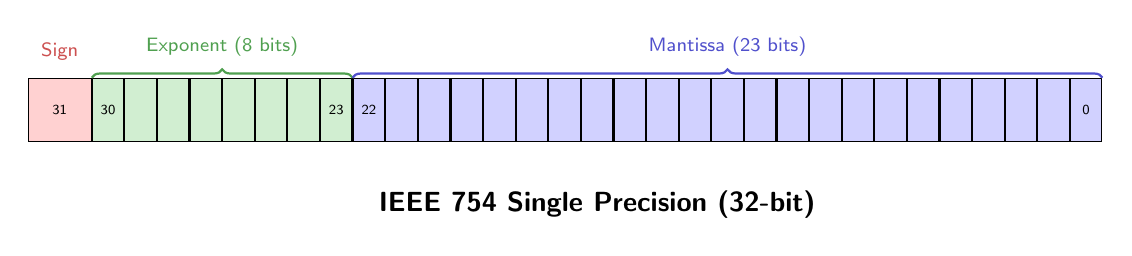
\begin{tikzpicture}[
    bitbox/.style={draw, minimum width=0.4cm, minimum height=0.8cm, inner sep=0pt, anchor=west, font=\sffamily\tiny},
    label/.style={font=\sffamily\small}
]

    % Define colors
    \definecolor{signcolor}{RGB}{255, 100, 100}
    \definecolor{expcolor}{RGB}{100, 200, 100}
    \definecolor{mantissacolor}{RGB}{100, 100, 255}

    % Sign bit (31)
    \node[bitbox, fill=signcolor!30, minimum width=0.8cm] (b31) at (0,0) {31};
    \node[above=0.1cm of b31, font=\sffamily\scriptsize, text=signcolor!80!black] {Sign};

    % Exponent bits (30-23)
    \foreach \i in {30,29,...,23} {
        \ifnum\i=30
            \node[bitbox, fill=expcolor!30, right=0pt of b31] (b\i) {\i};
        \else
            \pgfmathsetmacro{\prev}{\i+1}
            \node[bitbox, fill=expcolor!30, right=0pt of b\prev] (b\i) {}; % hide numbers for middle bits to save space/clutter
        \fi
    }
    % Label for Exponent
    \draw[decorate, decoration={brace, amplitude=3pt}, thick, expcolor!80!black] (b30.north west) -- (b23.north east) node[midway, above=4pt, font=\sffamily\scriptsize] {Exponent (8 bits)};
    \node[font=\sffamily\tiny] at (b23) {23}; % show last bit index

    % Mantissa bits (22-0)
    \foreach \i in {22,21,...,0} {
        \ifnum\i=22
            \node[bitbox, fill=mantissacolor!30, right=0pt of b23] (b\i) {\i};
        \else
            \pgfmathsetmacro{\prev}{\i+1}
            \node[bitbox, fill=mantissacolor!30, right=0pt of b\prev] (b\i) {};
        \fi
    }
    % Label for Mantissa
    \draw[decorate, decoration={brace, amplitude=3pt}, thick, mantissacolor!80!black] (b22.north west) -- (b0.north east) node[midway, above=4pt, font=\sffamily\scriptsize] {Mantissa (23 bits)};
    \node[font=\sffamily\tiny] at (b0) {0}; % show last bit index

    % General Label
    \node[below=0.5cm of b15, font=\bfseries\sffamily] {IEEE 754 Single Precision (32-bit)};

\end{tikzpicture}

\end{document}
